\section{Extra-Vehicle Car-to-X (C2X) Networking}

La suddivisione dei casi d'uso della comunicazione tra veicoli e tutto il resto (V2X) si compone
nella seguente maniera:

\begin{itemize}
	\item \textbf{NON-SAFETY}: comunicazione non legata alla sicurezza
	      \begin{itemize}
		      \item Comfort
		      \item Informazione traffico
	      \end{itemize}
	\item \textbf{SAFETY}: comunicazione legata alla sicurezza
	      \begin{itemize}
		      \item Situation awareness
		      \item Warning messages
	      \end{itemize}
\end{itemize}



\subsection{Motivazioni}

\begin{itemize}
	\item Traditional Network: \textbf{wired, non mobile, static}
	\item Mobile Ad-Hoc Network:(MANET) \textbf{wireless, mobile, dynamic}
	\item Vehicular Ad-Hoc Network: (VANET) \textbf{wireless, mobile, dynamic}
\end{itemize}

Da notare la differenza fra guida in centri urbani e guida su super strada, ci sono pro e contro
introdotti da ciascuna casistica.


\subsection{Livelli di supporto infrastrutturale}

\begin{itemize}
	\item Pure ad-hoc communication
	\item Stationary Support Unit (SSU)
	\item Road Side Unit (RSU)
	\item Traffic Information Center(TIC)
\end{itemize}

Si tende a preferire un'approccio eterogeneo per sfruttare i vantaggi di una comunicazione con e
senza infrastruttura.

\subsection{Le sfide della comunicazione C2X}



\subsubsection{Comunicazione}
\begin{itemize}
	\item Condizioni del canale fortemente variabili.
	\item Alta congestione, contesa, interferenza.
	\item Capacità del canale fortemente limitata.
\end{itemize}

\subsubsection{Networking}
\begin{itemize}
	\item Collegamenti unidirezionali.
	\item Necessità di multi-radio e multi-rete.
	\item Apparecchiature eterogenee.
\end{itemize}

\subsubsection{Mobilità}
\begin{itemize}
	\item Topologia altamente dinamica.
	\item Tuttavia, mobilità prevedibile.
	\item Ambiente eterogeneo.
\end{itemize}

\subsubsection{Sicurezza}
\begin{itemize}
	\item Nessun collegamento affidabile all'infrastruttura centrale.
	\item Garantire la privacy.
	\item Base di utenti eterogenea.
\end{itemize}


\section{Paradigmi di comunicazione}

\begin{figure}
	\centering
	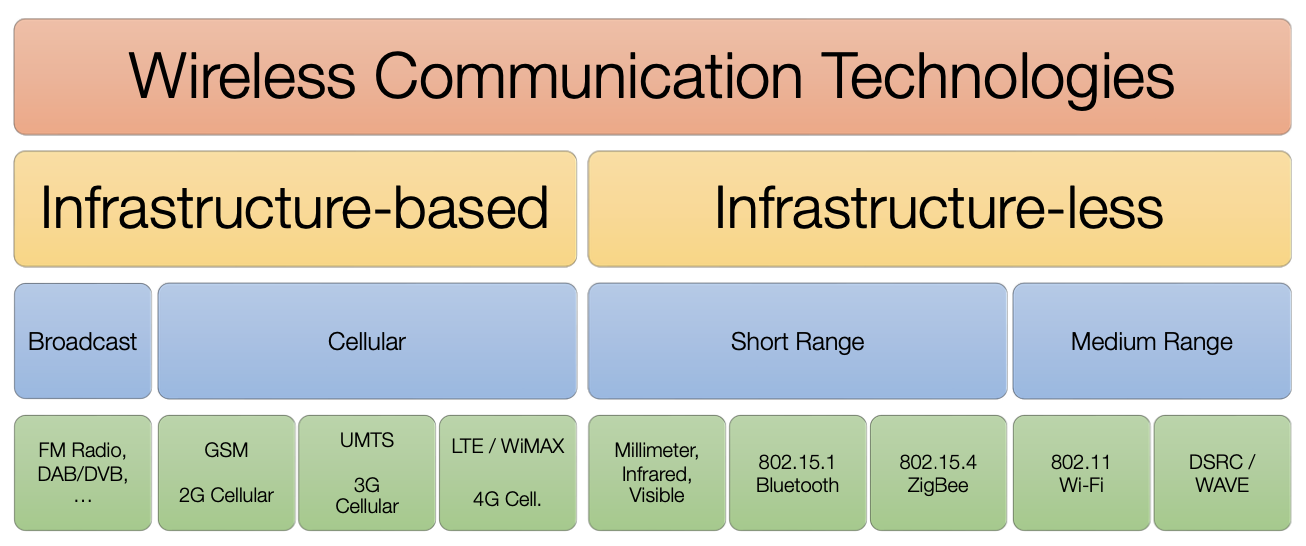
\includegraphics[width=0.7\textwidth]{images/paradigmi.png}
\end{figure}


La comunicazione wireless si divide in due macro categorie: \textbf{basata su infrastruttura} e
\textbf{non basata su infrastruttura}.

I paradigmi basati sull'utilizzo di una infrastruttura sono:
\begin{itemize}
	\item Broadcast
	\item Cellular
\end{itemize}

Per quanto riguarda la comunicazione non basata su infrastruttura abbiamo:
\begin{itemize}
	\item Short range
	\item Medium range
\end{itemize}


\subsection{Broadcast media}
\subsubsection{Traffic Message Channel (TMC)}

Gestione centralizzata delle informazioni del traffico, le informazioni provengono da vari canali
federali Americani.

Le informazioni sono codificate per avere un significato basato sulla posizione geografica, si
compongono tabelle regionali che rappresentano il codice dell'evento e il suo significato.


\subsubsection{Transport Protocol Experts Group (TPEG)}

Successore pianificato di TMC, fondato sui seguenti principi:
\begin{itemize}
	\item Espandibilità
	\item Indipendeza dal media di trasmissione
\end{itemize}


Gli obietti di TPEG sono:
\begin{itemize}
	\item Costruire il sistema alla base per \textbf{Digital Audio Broadcast (DAB)}
	\item Modulare
	\item Broadcast(mono directional) e point-to-point (multi directional)
	\item integra sicurezza mediante il CRC(Cyclic Redundancy Check)
\end{itemize}


\subsection{Cellular Networks}

Il concetto alla base dell'utilizzo della rete cellualre \`e quello di dividere il mondo in tanti
esagoni che sono le celle, ogni cella viene servita da una stazione.


L'utilizzo delle celle impone una forte gerarchia nella rete, poich\`e dopo le celle si incanalano
nella backbone del paesino, poi del paese, poi della nazione e cosi via.

\subsubsection{UMTS(3G)}

Perdita di segnale se a 290 $km/h$ si effettua una frenata brusca ma i veri problemi sono legati
alla latenza e alla capacità della rete.

Ci sono due metodologie della gestione dei canali con UMTS:
\begin{itemize}
	\item Shared channel: Random Access Channel (RACH) in uplink e il Forward Access Channel (FACH)
	      in downlink.
	\item Dedicated Transport Channel (DCH)
\end{itemize}


Nello specifico \textbf{FACH} gli slot temporali sono gestiti dalla stazione base, il ritardo si
aggira intorno ai 10 $ms$.

\textbf{RACH} ha un ritardo approssimativo di 50 $ms$ e utilizza ALOHA(che non è un protocollo di
controllo di accesso al mezzo) per la gestione dei canali.

\textbf{DCH} ha un ritardo di 250 $ms$ oppure 2 $s$ oppure 10 $s$ per l'attivazione del canale,
mantenere la comunicazione in DCH \`e molto costoso.



\subsection{IEEE 802.11p}

La tecnologia proposta dallo standard IEEE 802.11p vuole integrare la tecnologia \textbf{WAVE}
(Wireless Access in Vehicular Environments) per la comunicazione tra veicoli e infrastrutture.

I contro principali sono:
\begin{itemize}
	\item Switching costoso
	\item Associazione costoso
	\item Sicurezza
	\item no QoS
	\item Poco range e poca velocità
\end{itemize}

Il layer fisico permetta comunicazione fino ad una distanza di 1 $km$ e una velocità di 200 $km/h$,

Solitamente lo standard IEEE 802.11p usa un'approccio di isolamento dei client rispetto al router
principale, questo approccio di tipo WAVE mi sembra pi\`u un'approccio ripreso dai prodotti IOT dove
ogni device fa da client e da relay del segnale, ogni comunicazione scorre attraverso i vari nodi.


Esiste un terzo approccio che prende il nome di WAVE BSS:
\begin{itemize}
	\item Nessuna separazione tra HOST e AP
	\item classificazione lasca in base all'hardware
	\item Possibilità di creare un beacon con tutti i parametri per joinare la rete
\end{itemize}


\subsection{UMTS/LTE vs IEEE 802.11p}

I pro di UMTS/LTE sono:
\begin{itemize}
	\item Servizio centralizzato
	\item Infrastruttura pre deployata
	\item Migrazione facile con telefoni
\end{itemize}

I contro di UMTS/LTE sono:
\begin{itemize}
	\item Latenza
	\item La rete necessita di essere dimensionata per supportare il traffico(upgrade)
	\item Servizio centralizzato
\end{itemize}

I pro di IEEE 802.11p sono:
\begin{itemize}
	\item poca latenza
	\item non sono necessari operatori di rete
	\item carico della rete distribuito
	\item privacy
\end{itemize}

\begin{itemize}
	\item necessita di un gateway in una RSU(Road Side Unit) per l'accesso alla rete(hardware da
	      implementare)
\end{itemize}


\subsection{CALM}
CALM (Communication Access for Land Mobiles) \`e un progetto che vuole integrare la tecnologia
basa su IEEE 802.11p con la tecnologia basata su LTE, integra:
\begin{itemize}
	\item WIFI
	\item WAVE
	\item ETHERNET
	\item altro
\end{itemize}

\subsection{IEEE 1609}

Standard on top of IEEE 802.11p, definisce:
\begin{itemize}
	\item Sicurezza
	\item Servizi di rete
	\item Gestione dei canali
	\item applicazione dei pagamenti digitali
\end{itemize}


\subsubsection{Gestione dei canali}

Sincronizza i canali mediante il clock di GPS e invia dati in slot temporali seguiti da un intervallo
di pause per permettere la ricezione dei dati da parte dei client.


\subsubsection{Gestione dei canali}
Due canali principali:
\begin{itemize}
	\item Control Channel (CCH)
	\item Service Channel (SCH)
\end{itemize}



Con lo standard IEEE 1609 utilizza WSA (Wave Service Announcement) per la gestione dei canali,
quindi la prima fase della comunicazione che si occupa di gestire i canali (CCH), esistono tanti codici per definire
come sar\`a la comunicazione (vehicle safety, emergency warning ecc..).

Dopo di che vengono utilizzati i canali di servizio (SCH) per la comunicazione vera e propria.


\subsubsection{Sicurezza}

La sicurezza è integrata in WAVE mediante firma, verifica e cifratura dei dati, inoltre si utilizza
un certificato che identifica il veicolo e questo deve essere rilasciato con diverse metodologie:
\begin{itemize}
	\item By role: CA, RSU, OBU
	\item By application: emergency, safety, payment
	\item By application priority: emergency, safety, payment
	\item By location and time
\end{itemize}


\subsection{ETSI ITS G5}
Standard Europeo per usare la tecnologia basata su IEEE 802.11p e WAVE.

Il cambiamento principale \`e la decentralizzazione del controllo di congestione,
DCC (Decentralized Congestion Control) \`e un protocollo che si occupa di gestire la congestione
mediante il controllo del numero di messaggi che si possono inviare in un intervallo di tempo.

La gestione dei canali non avviene in maniera alternata ma in maniera concorrente, quindi il CCH
ha un canale dedicato e il SCH ha un canale dedicato.

CCH ora ha:
\begin{itemize}
	\item SAM: Service Announcement Message
	\item CAM: Cooperative Awareness Message
	\item DENM: Decentralized Environmental Notification Message
\end{itemize}

Mentre SCH pu\`o trasportare i dati delle applicazioni.

\subsection{Routing: Broadcast, Geocast, Routing}

Approccio classico:
\begin{itemize}
	\item Distance Vector Routing: Ogni nodo conserva informazioni sulle distanze verso i vicini
	\item Link State Routing: Ogni nodo conosce la topologia della rete
	\item Reactive(on demand) Routing: Il percorso viene calcolato solo quando necessario
	\item Proactive Routing: Il percorso viene calcolato periodicamente
	\item Hop-by-hop Routing: Il percorso viene calcolato nodo per nodo
	\item Source Routing: Il percorso viene calcolato dal nodo sorgente
	\item Georouting: Il percorso viene calcolato in base alla posizione geografica
\end{itemize}




\subsection{Flooding}

Il flooding \`e un metodo di routing che consiste nell'inviare un messaggio a tutti i nodi della
rete, questo metodo \`e molto costoso e non \`e efficiente.

Le soluzioni per migliorare il flooding sono:
\begin{itemize}
	\item Flooding probabilistico
	\item Scambio di informazioni con vicino
	\item Creazione di una topologia
\end{itemize}


Per VANET \`e stato scelto un approccio che sopprime i messaggi duplicati, questo approccio
ha dei pro:
\begin{itemize}
	\item Servono informazioni dei vicini
	\item massimizza la distanza tra nodi
	\item Minimizza perdita di messaggi
\end{itemize}




\subsection{DV-Cast}

Ogni nodo invia periodicamente un beacon di saluto contenente:
\begin{itemize}
	\item Posizione
	\item Velocità
\end{itemize}

Ogni nodo gestisce 3 tabelle di vicini:
\begin{itemize}
	\item stessa direzione e davanti
	\item stessa direzione e dietro
	\item direzione opposta
\end{itemize}

\subsection{GeoCast}

I nodi mandano un beacon di saluto e la gerachia della rete rispecchia le distanze del mondo reale,
ogni nodo conosce fino a due salti nella rete.


\subsection{Svantaggi}
\begin{itemize}
	\item Classic information dissemination:
	      \begin{itemize}
		      \item Distance vs link state
		      \item Proactive vs reactive
		      \item Hop-by-hop vs source
		      \item Georouting
	      \end{itemize}
	\item VANET:
	      \begin{itemize}
		      \item Flooding
		      \item Fragmentation(DV-Cast)
		      \item Directedness(To GO)
	      \end{itemize}
	\item Scalabilità
\end{itemize}


\subsection{Beaconing and TIS – Traffic Information Systems}

Obiettivo quello di:
\begin{itemize}
	\item Miglior confort
	\item ridurre code
	\item ridurre tempi percorrenza
	\item scorrimento del traffico smooth
	\item Meno emissioni
\end{itemize}

\subsubsection{SOTIS}
SOTIS (Self Organizing Traffic Information System):
\begin{itemize}
	\item Ogni nod oha una conoscenza locale
	\item manda single hop broadcast con informaioni periodicamente
	\item Integra informazioni nuove nella sua conoscenza locale
\end{itemize}

\subsubsection{ATB}
ATB (Adaptive Traffic Beaconing):
\begin{itemize}
	\item Uso elastico della infrastruttura
	\item uso di read side unit (RSU)
\end{itemize}


